Formally evaluating the effectiveness of a meta-toolkit for visual
analytics is complex. Arguably the most convincing method would
require two groups of programmers of equivalent skills to implement
the same set of visual analytics programs with and without
Obvious. Then, a judgment could be made from the time spent and the
quality of the results. This methodology has been used to assess the
InfoVis Toolkit~\cite{InfoVis} with students but is impractical for
real Visual Analytics applications that are more complex and would not
fit the scope of student projects.

Another method --- used to validate Prefuse~\cite{Prefuse} -- would be
to re-implement complex Visual Analytics applications using Obvious
and assess the results, again in term of time and quality. This is
what we have done and we report on our results here.

\subsection{Coding applications with Obvious}

This section shows how Obvious can implement common applications in
information visualization such as the creation of a scatter-plot or of
a network visualization.  These examples explain how to combine
Obvious components to build an application, how to create data
structure and spot patterns to use.  The first use-case concerns the
coding of a network visualization with the Obvious-InfoVis Toolkit
implementation and the second based on the coding of a scatter-plot by
combining component from different Obvious implementations.

For both examples and more generally for every creation of an Obvious
application, developers have to follow the following steps:
\begin{itemize}
\item Creation of an Obvious data structure, either directly with a
  standard constructor or through a factory.  Three ways exist to fill
  the data structure:
  \begin{enumerate}
  \item wrapping an existing data structure from a targeted toolkit as
    shown in the first example,
  \item using an Obvious reader to load an Obvious structure from a
    well known file format (CSV, GraphML...) as shown in the second
    example,
  \item using Obvious methods to directly manipulate the data
    structure (addRow, addNode, addEdge...); an example would be too
    long for this article.
 \end{enumerate}

\item Creation of an Obvious visualization from the created data
  structure and additional parameters.  This can be done directly with
  a class constructor or through a factory.  The parameters allow
  customization of the Obvious monolithic components.  As shown in the
  second example, it is possible to use the data structure from
  one Obvious implementation with a visualization from another.

 \item Creation of an Obvious view with the created visualization
   directly with a constructor or through a factory
\end{itemize} 

\begin{lstlisting}[caption={Visualizing a graph with Obvious},label=codeSample1]
// Creates the graph structure. First, set the factory to use (ivtk).
// Then load the native data structure, and get a factory instance.
// Finally, call the convenient getter of the factory.
System.setProperty("obvious.DataFactory",
    "obvious.ivtk.data.IvtkDataFactory");
infovis.Graph g = Algorithms.getGridGraph(10, 10);
DataFactory factory = DataFactory.getInstance()
Network network = factory.createGraph(g);

// Creates the associated visualization using the
// factory for visualization. No predicate and extra
// parameters are given to the constructor.
Visualization vis = new IvtkVisualizationFactory()
    .createVisualization(network, null, "network", null);

// Creates the view. No predicates and extra parameters are given to
// the constructor.
View view = new IvtkObviousView(vis, null, "graphview", null);
// Standard Java window creation
JFrame frame = new JFrame();
JScrollPane panel = new JScrollPane(view.getViewJComponent());
frame.add(panel);
frame.pack();
frame.setVisible(true);
\end{lstlisting}

\begin{lstlisting}[caption={Combining different Obvious implementations to display a scatter-plot},label=codeSample2]
// Defining the data factory to use,
// obvious-prefuse will be used for the data structures.
System.setProperty("obvious.DataFactory",
    "obvious.prefuse.PrefuseDataFactory");
// Creating an Obvious CSV reader and loading an
// Obvious table
CSVImport csv = new CSVImport(new File("example.csv"), ',');
Table table = csv.loadTable();

// Creating the parameter map for the monolithic object.
Map<String, Object> param = new HashMap<String, Object>();
param.put("x", "id"); // xfield
param.put("y", "age"); // yfield

// Creating the visualization then the view. No predicates are given to
// the constructor.
Visualization vis = new IvtkScatterPlotVis(table, null, "plot", param);

View view = new IvtkObviousView(vis,  null, "plot", null);
// Standard Java window creation
...
\end{lstlisting}

\subsection{Integration of Weka}

Weka~\cite{Weka} is a suite of machine-learning algorithms and data
structures widely used to design machine-learning applications.  
The obviousx package of Obvious supports two mechanisms to build the
main data structure of Weka (called ``Instances'') from an Obvious
Table:

\begin{itemize}
\item an Obvious table can be copied into a Weka ``Instances'', which
  is a data structure specially optimized for fast processing with
  clustering and machine learning algorithms.  With this approach,
  running-time is optimized.
\item an Obvious table can wrap a Weka ``Instances'': the Obvious
  table translates its methods into the Weka equivalents.  With this
  approach, memory-consumption is optimized.
\end{itemize}

Both methods are equivalent in terms of lines of code and can be
applied to the same machine learning algorithms from Weka.  For
example, wrapping the table from the code sample \ref{codeSample2}
into a Weka ``Instances''  requires the following line:

\begin{lstlisting}[caption={Wrapping an Obvious Table into Weka Instances},label=wekaExample]
Instances inst = new ObviousWekaInstances(table, "Instances");
\end{lstlisting}

%% To wrap the Obvious structure, the constructor simply needs as
%% argument the Obvious table and a name for the weka Instances.  

This ``Instances'' can be used by all the machine-learning algorithms
defined in Weka.  Creating this wrapper took about three days to one
developer who knew Obvious well but was discovering Weka.

This example demonstrates an important gain of Obvious: a toolkit with
a binding in Obvious can immediately benefit from a substantial set of
additional features, such as Weka for advanced machine-learning
capabilities and several format converters.  Conversely, developers of
new analysis algorithms could port them to use Obvious data structures
to become usable by a substantial number of toolkits and application
programmers to build visual analytics systems.


\subsection{EdiDuplicate}

EdiDuplicate is a system built with Obvious, designed to detect and
merge duplicated entities in the HAL publication database. It is an
adaptation of the D-Dupe software~\cite{DDupe} written in .NET.  To
help resolve the entities, two types of information are visualized:
the similarity measures between entities to resolve and the social
network of these entities, as shown in Figure~\ref{fig:ediduplicate}.

Each time a new entity is created in the HAL database, a module
computes multiple similarity metrics from this entity to all the ones
already in the database.  This information is loaded on an Obvious
table and displayed on the left pane using a standard Java table. Each
row refers to one pair of names and the columns contain the multiple
similarity measures with a green-red color coding; the table that can
then be sorted according to any column order.

When pair is selected by clicking on a row, a network view is created
on the right visualizing the neighborhood network of the pair of
entities.  This neighborhood is computed from publication data: for a
target entity, it contains all the entities already connected to it
through co-authorship relations.  This information helps the user
decide if the pair of entities has to be merged.

\begin{comment}
INRIA, the French National Institute of Research in Computer Science
and Control, maintains an repository called
HAL-INRIA\footnote{\url{http://hal.inria.fr}} to store, index and give
access to its publications.  Entering publications is a manual process
done by researchers who make mistakes.  These mistakes can result in
duplicated authors, institutions, or articles (HAL treats two entities
as different when they are the same). Thus, INRIA needs to clean the
HAL database with tools that can detect potential duplicates and ask
skilled users to resolve them by either unifying them or confirming
that they are different.  Currently, INRIA leaves that task to
librarians with very primitive tools.

This problem has already been addressed by at least two communities:
the database community, which calls it the ``Record Linkage'' or
``Entity Resolution'' problem, and the Visual Analytics community with
the D-Dupe tool~\cite{DDupe}.  D-Dupe uses similarity metrics between
entity names and information visualization techniques to show a rich
set of information to the librarian to make a decision whether two
entities are the same or different.  However, since D-Dupe does not
connect to the workflow of HAL, we used Obvious to build a similar
tool that we called EdiDuplicate.
\end{comment}

\begin{figure}[!h]
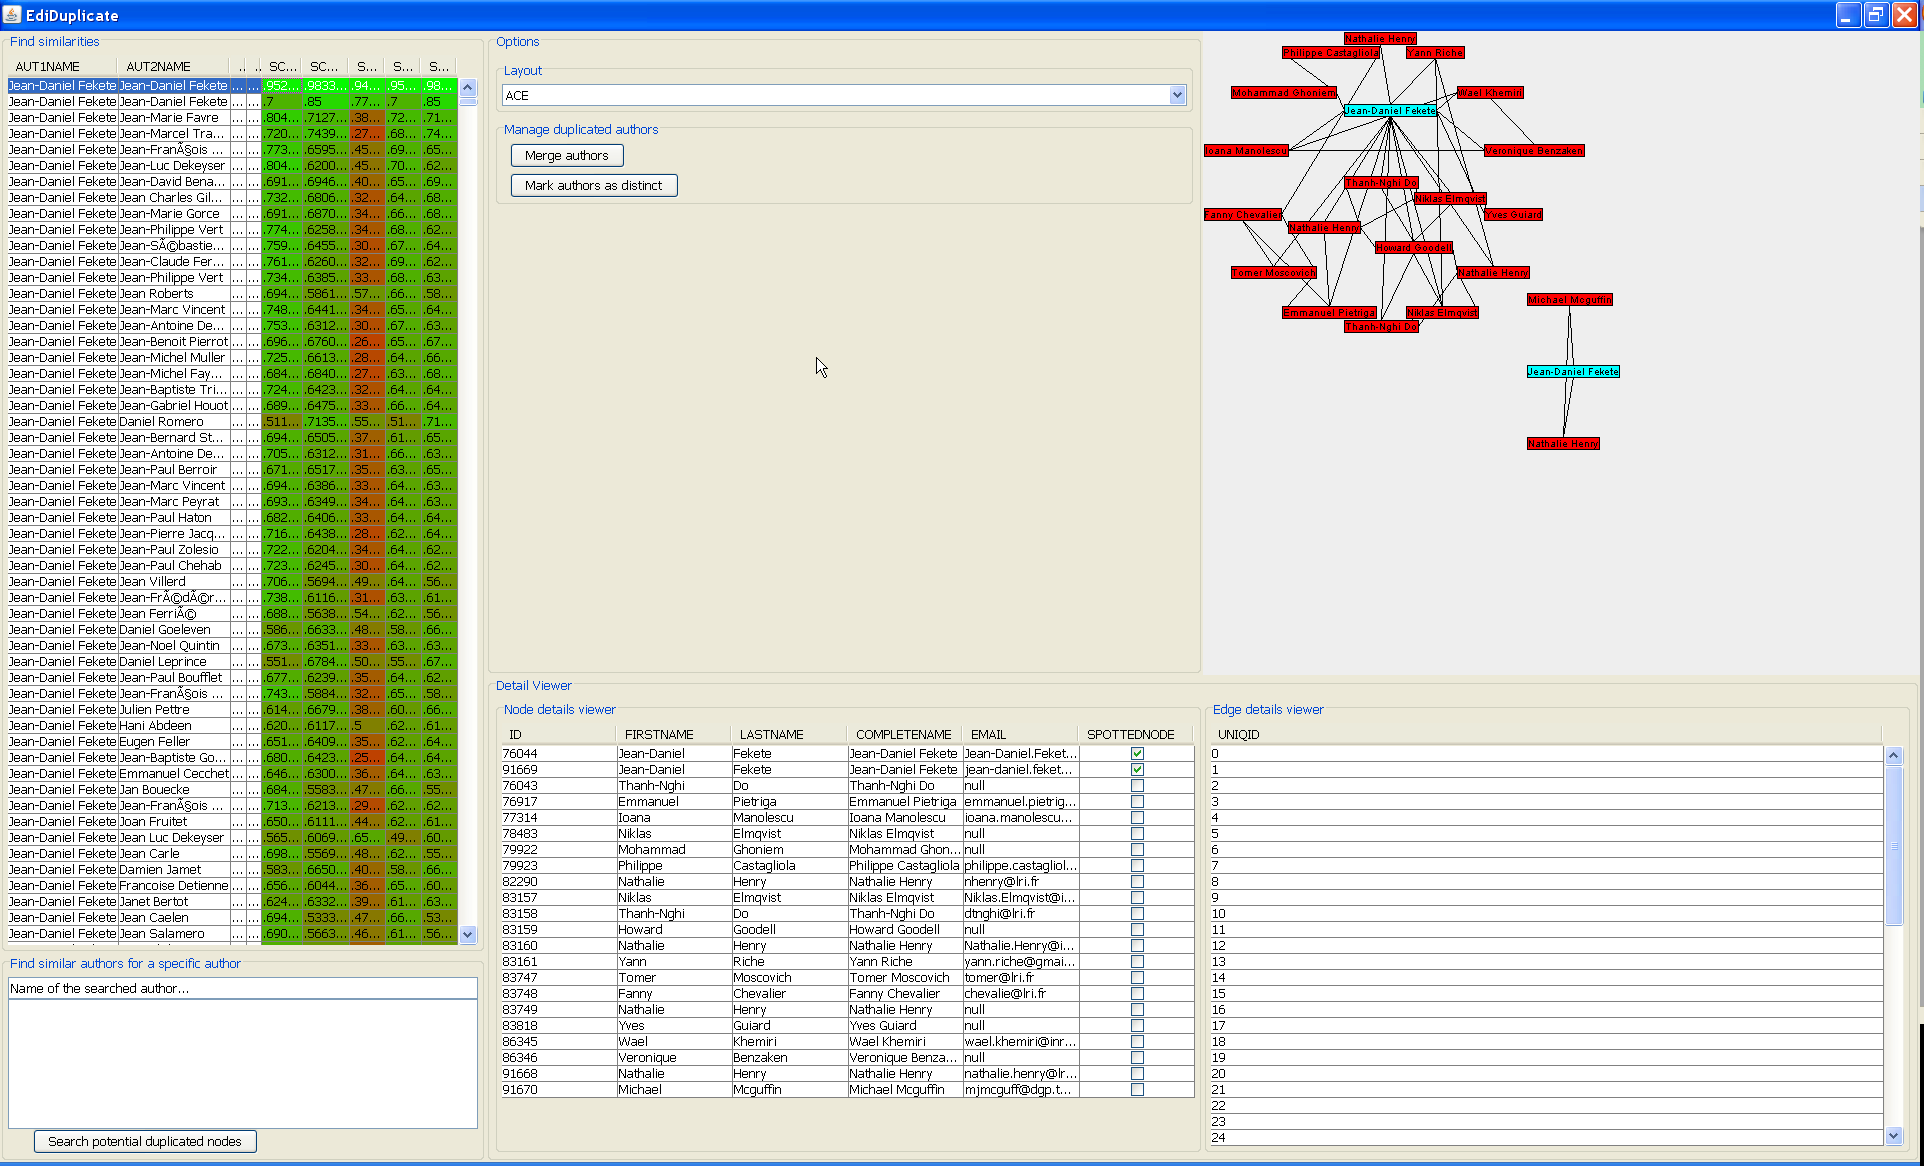
\includegraphics[width=\columnwidth]{figures/ediduplicate}
\caption{The EdiDuplicate application}
\label{fig:ediduplicate}
\end{figure}

EdiDuplicate offers the same features than D-Dupe but with extensions
to cover needs specific the INRIA-HAL
database\footnote{\url{http://hal.inria.fr}}. The application mainly
combines Obvious components and Swing components (derived from Obvious
structures). For the data model, an Obvious Network is used using the
InfoVis Toolkit implementation of Obvious; the visualization and the
view parts are also provided by this implementation.  Building this
application took less than a week.

\subsection{DBMS Caching Data Table}
\label{dbmscachingtable}

The need to create DBMS caching data table appears during the development
of Ediflow, a Scientific Workflow system for Visual Analytics \cite{Ediflow}.
Ediflow is organized around a DBMS (Oracle) and runs modules processing
large amount of data stored in the DBMS. Ediflow is a distribued system
allowing workflows to be shared on several platforms.

When running a visualization component with Ediflow, all its resulting
visual attributes are stored in a table of the DBMS called
``VISUALATTRIBUTES''. This table is then used to create and maintain
views on other platforms using Ediflow.

To set up and maintain thoses view, in-memory caching tables are needed
to only select in ``VISUALATTRIBUTES''  data useful for those views
and to locally store it.

Those cached tables are implemented using Obvious (different bindings
have been used Prefuse, Infovis and JUNG). Not only Obvious cached
tables stores store data from ``VISUALATTRIBUTES'' but also they are
synchronized with it.

The Oracle DBMS has been extended to trigger notifications when
``VISUALATTRIBUTES'' changes (data are added, removed or updated). Those
notifications are received by Obvious cached tables that update their
content and launch recomputing of their layout.

Several applications has been built around Obvious DBMS caching
tables. They are introduced in \cite{Ediflow}. One of this application
is presented in the next section.

\subsection{Large Wall Network Visualization}

INRIA owns a large wall of 32 display screens
\footnote{\url{http://www.lri.fr/~mbl/WILD/}}. An application using it
has been developped to visualize with Obvious a large network visualization
of the co-authorship graph of INRIA. The idea is to create a visualization
component loaded on the 16 machines composing the wall, each component
displaying a part of this social network.

An Oracle DBMS stores publications data in two tables : one for the author
(containing id and name) and one for publications (containing pairs
of publication id and author id).

The first step is to calculate visual attributes to complete the
``VISUALATTRIBUTES'' table introduced in \ref{dbmscachingtable}.
This is done by a program that creates an Obvious network from
the authors and publications tables of the DBMS. Once the network is filled,
an Obvious visualization component from the Prefuse binding computes visual
attributes and they are written into the corresponding table of the
DBMS.

Then, on each machine of the wall a DBMS caching table linked to
``VISUALATTRIBUTES'' is loaded. This cached table contains the data
located in the portion of the screen that the machine has to display.
Then, corresponding visualizations and views are built from those
cached tables with component from the Prefuse binding.

Since cached tables are synchronized with the DBMS when the visual
attributes table of the DBMS is changed, the layout of the graph is
recomputed and changes appear on the wall.

\subsection{Implementing a Cross-Toolkit Layout Component}

We have also tested a more advanced usage scenario: devising
a novel layout algorithm and using the Obvious toolkit to make it
available in a variety of toolkits. This layout component is a
generalized treemap algorithm.
%% ~\cite{Treemaps2011}.  [jdf: not yet]
Its interface makes it easy to port as this
algorithm takes as input a data model and renders using a Visitor
design pattern to a renderer object, making it very convenient to
implement across polylithic toolkits such as Prefuse or Discovery.
Considering that the current visualization model is mostly targeted at
enabling monolithic patterns, Obvious in its current state turns out
to be of limited use for our purpose.

Still, we have found that the existing data model and utilities have
made developing our layout algorithm on top of Obvious worthwhile: we
could implement very easily a simple monolithic visualization and
view instances, and relying on the default data model already saves us
time in the development of our prototype, while we have the assurance
that only minimal work may be needed to port our method to the
toolkits targeted by Obvious.


\subsection{Conclusion}

The examples described in this section assess an important strength of
Obvious: it allows a clear separation of concerns in the development
of visual analytics applications with a small memory and performance
footprint.  The data model of the application can be chosen
independently from the visualization components as long as all these
components fit the Obvious model.  From our experience, a large number
of the visual analytics application fit the Obvious model and they
will benefit from the meta-toolkit in term of richness and
extensibility.

